\documentclass[hyperref={xetex}]{beamer}
\title{Einführung in Matlab und Python - Einheit 3}
\subtitle{Rekursionen, Grafik}
\mode<article>
{
  \usepackage{fullpage}
  \usepackage{pgf}
  \usepackage{hyperref}
  \setjobnamebeamerversion{beamer}
}

\mode<presentation>
{
  %\usetheme{Frankfurt}
 %\usetheme{My}
  \usetheme{Madrid}
  % or ...
%\usecolortheme{seagull}
  %\setbeamercovered{transparent}
  %\setbeamercovered{dynamic}
  % or whatever (possibly just delete it)
}
\usenavigationsymbolstemplate{}
\usefonttheme{structurebold}
\usepackage{multimedia}
\usepackage{tikz}
\usepackage{fontspec,xunicode,xltxtra}
%\usepackage[scaled=.90]{helvet}
% Or whatever. Note that the encoding and the font should match. If T1
% does not look nice, try deleting the line with the fontenc.

\setbeamertemplate{footline}
{
\leavevmode
%\hbox{\begin{beamercolorbox}[wd=.5\paperwidth,ht=2.5ex,dp=1.125ex,
%leftskip=.3cm plus1fill,rightskip=.3cm]{author in head/foot}%
%    \usebeamerfont{author in head/foot}\insertshortauthor
%  \end{beamercolorbox}%
%  \begin{beamercolorbox}[wd=.5\paperwidth,ht=2.5ex,dp=1.125ex,leftskip=.3cm,
%rightskip=.3cm plus1fil]{title in head/foot}%
%    \usebeamerfont{title in head/foot}\insertshorttitle\hfill

\hfill\insertframenumber  \hspace{3pt}

%\inserttotalframenumber
%\hspace*{2ex}
%  \end{beamercolorbox}}%
  \vskip3pt%
}

%\usepackage[english]{babel}
\usepackage[ngerman]{babel}
\selectlanguage{ngerman}

%
% math/symbols
%
\usepackage{amssymb}
\usepackage{amsthm}
% \usepackage{latexsym}
\usepackage{amsmath}
%\usepackage{listings}
\usepackage[framed]{mcode}
%\usepackage{mcode}

\usepackage{mydef}
\usepackage{cmap} % you can search in the pdf for umlauts and ligatures
%\usepackage{colonequals} %corrects the definition-symbols \colonequals (besides others)
\title{Einführung in Matlab}
%
%\subtitle{Disputation} % (optional)

\author{Jochen Schulz}
% - Use the \inst{?} command only if the authors have different
%   affiliation.

\institute{Georg-August Universit\"at G\"ottingen \pgfimage[height=0.5cm]{../figures/unilogo3}}
% - Use the \inst command only if there are several affiliations.
% - Keep it simple, no one is interested in your street address.

\date{\today}

\subject{Einführung in Matlab}
% This is only inserted into the PDF information catalog. Can be left
% out. 



% If you have a file called "university-logo-filename.xxx", where xxx
% is a graphic format that can be processed by latex or pdflatex,
% resp., then you can add a logo as follows:

%\logo{\pgfimage[height=0.5cm]{figures/unilogo3}}


% Delete this, if you do not want the table of contents to pop up at
% the beginning of each subsection:
% \AtBeginSubsection[]
% {
%   \begin{frame}<beamer>
%     \frametitle{Aufbau}
%     \tableofcontents[currentsection,currentsubsection]
%   \end{frame}
% }

\AtBeginSection[]
{
  \begin{frame}<beamer>
    \frametitle{Aufbau}
    \tableofcontents[currentsection,currentsubsection]
  \end{frame}
}


\begin{document}



\begin{document}
\titlepage


\section{Rekursionen}
%
% Slide
%
\begin{frame}[fragile]{Rekursive Funktionen}
Rekursive Funktionen sind Funktionen, die sich selbst aufrufen.\\
Bei jedem Aufruf wird ein neuer lokaler Workspace erzeugt.\\[1cm]

\textbf{Beispiel:} Fakult"at: $n!=\fak(n)$\\
\begin{eqnarray*}
 n!& = & n(n-1)!=n \fak(n-1)\\
& = & n(n-1)\fak(n-2)\\
& = & \cdots= n(n-1)\cdots 1 
\end{eqnarray*}
\end{frame}
%
% Slide
%
\begin{frame}[fragile]{Fakult"at - rekursiv}
\matinput{fak.m}
\begin{pyin}
def fak(n):
    if (n == 1):
        res = 1
    else:
        res = n*fak(n -1)
    return res
\end{pyin}
\end{frame}
%
% Slide
%
\begin{frame}[fragile]{Fakult"at - direkt}
\matinput{fak_it.m}
\begin{pyin}
def fak_it(n):
    fak = 1
    for i in range(1,n+1):
        fak = fak*i
    return fak
\end{pyin}
\end{frame}
%
% Slide
%
\begin{frame}[fragile]{Fakult"at - Zeitvergleich}
\matinput{fak_vergleich.m}
\begin{pyin}
%timeit fak_it(20)
\end{pyin}
\end{frame}
%
% Slide
%
\begin{frame}[fragile]{rekursive Implementierung GGT}
\begin{matlabin}
function [a,b] = ggt_rekursiv(a,b)
if a~=b
  if a>b
    a = a-b;
  else
    b = b-a;
  end;
  [a,b] = ggt_rekursiv(a,b);
end;  
\end{matlabin}
\begin{pyin}
def ggt_rekursiv(a,b):
    if a != b:
        if a>b:
            a -= b
        else:
            b -= a
        return ggt_rekursiv(a,b)
    return a
\end{pyin}
\end{frame}
%
% Slide
% 
\begin{frame}[fragile]{Sierpinski Dreieck}
\begin{itemize}
\item Wir beginnen mit einem Dreieck mit Eckpunkten $P_a$, $P_b$ und $P_c$. 
\item Wir entfernen daraus das Dreieck, das durch die Mittelpunkte der
  Kanten entsteht.
\item Die verbliebenden drei Dreiecke werden der gleichen Prozedur
  unterzogen.
\item Diesen Prozess können wir rekursiv wiederholen.
\item Das Ergebnis ist das Sierpinski Dreieck.
\end{itemize}
\end{frame}
%
% Slide
% 
\begin{frame}[fragile]{Sierpinski Dreieck}
\begin{minipage}{5cm}
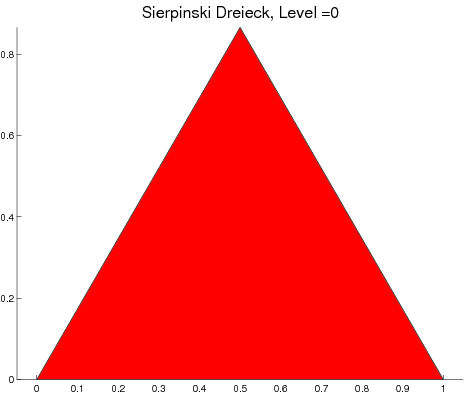
\includegraphics[height=4cm]{figures/sierpinski_0}
\end{minipage} \hfill
\begin{minipage}{5cm}
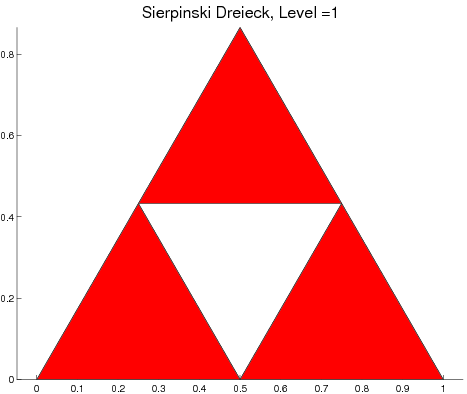
\includegraphics[height=4cm]{figures/sierpinski_1}
\end{minipage}\\ 
\begin{minipage}{5cm}
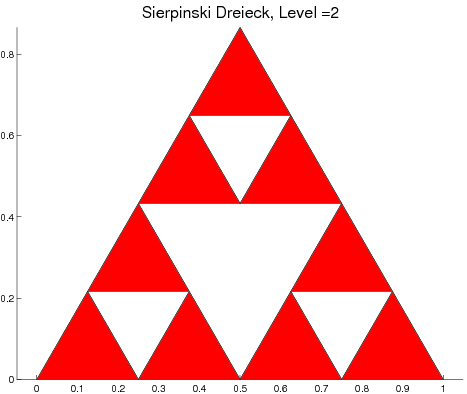
\includegraphics[height=4cm]{figures/sierpinski_2}
\end{minipage} \hfill
\begin{minipage}{5cm}
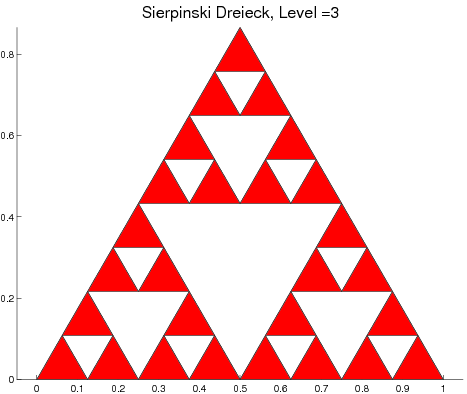
\includegraphics[height=4cm]{figures/sierpinski_3}
\end{minipage} \\
\end{frame}
%
% Slide
%
\begin{frame}[fragile]{Matlab: Implementierung}
\matinput{sierpinski_plot.m}
\end{frame}
\begin{frame}[fragile]{Matlab: Implementierung}
\matinput{sierpinski.m}
\end{frame}
% 
% Slide
% 
\begin{frame}[fragile]{Zeichnen von Polygonen}

Ein Polygon sei durch die Eckpunkte $(x_i,y_i)_{i=1}^n$ gegeben. Dann
kann durch den Befehl
\begin{matlabin}
fill(x,y,char)
\end{matlabin}
dargestellt werden. \imatlab{char} gibt die Farbe des Polygons an, z.B. rot
wäre \imatlab{'r'}.
\end{frame}
%
% Slide
%
\begin{frame}[fragile]{Python: Implementierung}
  \begin{pyin}
level = 1
ecke1 = array([0,0])
ecke2 = array([1,0])
ecke3 = array([0.5, sqrt(3)/2])
figure
sierpinski (ecke1 ,ecke2 ,ecke3 , level)
title ('Sierpinski Dreieck , Level ={}'.format(level))    
  \end{pyin}
\end{frame}
\begin{frame}[fragile]{Python: Implementierung}
  \begin{pyin}
def sierpinski(ecke1,ecke2,ecke3,level):
    """Teilt das Dreieck auf in 3 Dreiecke (level >0) 
    Plotten des Dreiecks ( level =0)"""
    if level == 0:
        fill ([ecke1[0],ecke2[0],ecke3[0]],[ecke1[1],ecke2[1],ecke3[1]],'r')
    else:
        ecke12 = (ecke1+ecke2)/2.
        ecke13 = (ecke1+ecke3)/2.
        ecke23 = (ecke2+ecke3)/2.
        sierpinski(ecke1,ecke12,ecke13,level-1)
        sierpinski(ecke12,ecke2,ecke23,level-1)
        sierpinski(ecke13,ecke23,ecke3,level-1)    
  \end{pyin}
\end{frame}


\section{Einf\"uhrung Grafik}
\subsection{einfache zweidimensionale Grafiken}
% 
% Slide
% 
\begin{frame}[fragile]{Standard-Plot}
\begin{matlabin}
plot(<x>,<y>)
\end{matlabin}
zeichnet für Vektoren $x=(x_1, \ \dots \ ,x_N)$ und  $y=(y_1, \dots \ ,y_N)$
eine Grafik, die die Punkte $(x_i,y_i)$ und $(x_{i+1},y_{i+1})$ miteinander
verbindet.

\begin{columns}[c]
 \column{0.45\textwidth}
\textit{Beispiel:}
\begin{matlabin}
x = linspace(0,2*pi,100);
y1 = sin(3*x);
plot(x,y1)
\end{matlabin}
 \column{0.5\textwidth}
\pgfimage[width=\textwidth]{figures/grafik_1}
\end{columns}
\end{frame}
% 
% Slide
% 
\begin{frame}[fragile]{Erweiterungen}
\begin{matlabin}
plot(<x>,<y>,<string>)
\end{matlabin}
\alert{String} besteht aus drei Elementen, die die Farbe, Linienstil
und die Markierung der Punkte kontrollieren. Die Reihenfolge der drei
Elemente ist beliebig.
\begin{columns}[c]
 \column{0.4\textwidth}
\textit{Beispiel:} Durch \\
\begin{matlabin}
plot(x,y,'r*--') 
\end{matlabin}
wird die Linie
gestrichelt (- -) in rot (r) gezeichnet und die Punkte durch *
markiert.
\column{0.55\textwidth}
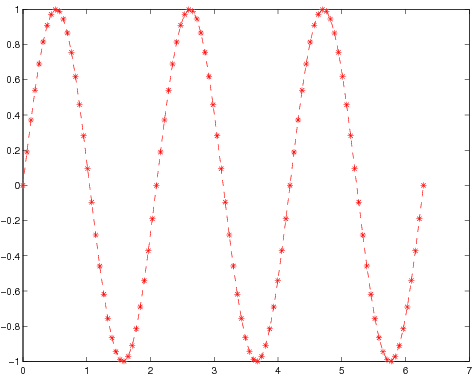
\includegraphics[width=\textwidth]{figures/grafik_2}
\end{columns}
\end{frame}
% 
% Slide
% 
\begin{frame}[fragile]{Optionen}
\begin{tabular}{cp{8.5cm}}
\alert{ Farben} & r (rot), g (grün), b (blau), c (hellblau), m (magenta),
  y (gelb), k (schwarz), w (weiß)\\
\alert{ Marker} & o (Kreis), * (Stern), . (Punkt), + (Plus), x (Kreuz), s
  (Quadrat), d (Raute),... \\
\alert{ Linien-Stil} &  - (durchgezogene Linie), \imatlab{--} (gestrichelte
  Linie), \imatlab{:} (gepunktete Linie), \imatlab{-.} (Strich-Punkt Linie)\\
\end{tabular}

Läßt man den Linien-Stil weg, so werden die Punkte nicht verbunden.
\end{frame}

% 
% Slide
% 
\begin{frame}[fragile]{Matlab: Optionen II}
\begin{matlabin}
plot(<x>,<y>,<string>,<Eigenschaft>, <Spez.>) 
\end{matlabin}
\alert{ Eigenschaften:}\\
\imatlab{'MarkerSize'} (Default 6), \imatlab{'LineWidth'} (Default 0.5),
\imatlab{'MarkerEdgeColor'}, \imatlab{'MarkerFaceColor'}\\

\begin{columns}[c]
 \column{0.6\textwidth}
\textit{Beispiel:} \\
\begin{matlabin}
plot(x,y1,'b-.d','LineWidth',...
3,'MarkerEdgeColor','g')
\end{matlabin}
\column{0.4\textwidth}
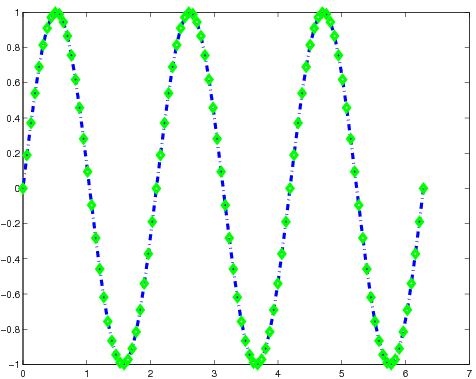
\includegraphics[width=\textwidth]{figures/grafik_3}
\end{columns}
\end{frame}
% 
% Slide
% 
\begin{frame}[fragile]{Alternativen}
\begin{itemize}
\item Mehrere Plots in eine Grafik:
\begin{matlabin}
plot(x1,y1,string1,x2,y2,string2,...) 
\end{matlabin}
\item Logaritmische Skalierung in $x$- bzw in $y$-Richtung:
\begin{matlabin}
semilogx(x1,y1) 
\end{matlabin}
  bzw. 
\begin{matlabin}
semilogy(x1,y1) 
\end{matlabin}
\item Logarithmische Skalierung beider Achsen: 
\begin{matlabin}
loglog(x1,y1)
\end{matlabin}
\item Ist $X$ ein Vektor mit komplexen Einträgen, so ergibt \alert{
  \imatlab{plot(X)}} 
\begin{matlabin}
plot(real(X),imag(X))
\end{matlabin}
\end{itemize}
\end{frame}
% 
% Slide
% 
\begin{frame}[fragile]{Beispiel - Legendre Polynome}
%\begin{columns}[c]
% \column{0.52\textwidth}
\begin{matlabin}[basicstyle=\scriptsize]
x = linspace(-1,1,100);
p1 = x;
p2 = (3/2)*x.^2-1/2;
p3 = (5/2)*x.^3-(3/2)*x;
p4 = (35/8)*x.^4 - (15/4)*x.^2+3/8;
plot(x,p1,'r:',x,p2,'g--',x,p3,'b-.',x,p4,'m-','LineWidth',2)
\end{matlabin}
%\column{0.48\textwidth}
\hfil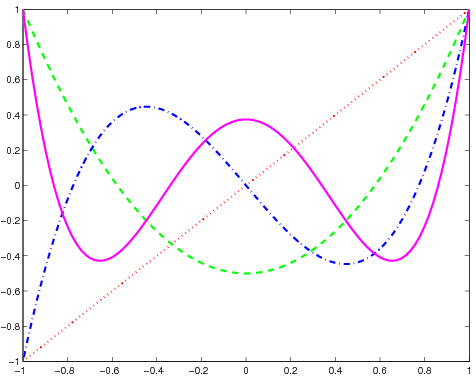
\includegraphics[width=0.55\textwidth]{figures/grafik_4}\hfil
%\end{columns}
\end{frame}
% 
% Slide
% 
\begin{frame}[fragile]{Achseneinstellungen}
\begin{tabular}{p{5cm}p{6cm}}
\imatlab{axis([x1 x2 y1 y2])} & Setzen der $x$- und $y$-Achsen
Grenzen\\
\imatlab{axis auto}| \isage{axis('auto')} & Rückkehr zu Default Achsen Grenzen\\
\imatlab{axis equal}| \isage{axis('equal')}& Gleiche Dateneinheiten auf allen Achsen\\
\imatlab{axis off}| \isage{axis('off')}& Enfernen der Achsen\\
\imatlab{axis square}| \isage{axis('square')}& quadratische Achsen-Box\\
\imatlab{axis tight}| \isage{axis('tight')}& Achsen Grenzen werden passend zu den Daten
gewählt. \\
\imatlab{xlim([x1 x2])} & Setzen der $x$-Achse\\
\imatlab{ylim([y1 y2])} & Setzen der $y$-Achse\\
\imatlab{grid on}| \isage{grid('on')} & Gitter aktivieren\\
\imatlab{box on}, \imatlab{box off}  | \isage{box('on')} \isage{box('off')}& Box um die Grafik
legen, Box entfernen
\end{tabular}
\end{frame}


\subsection{Beschriftungen}
% 
% Slide
% 
\begin{frame}[fragile]{Beschriften der Grafik}
\begin{itemize}
\item Titel:  \alert{ \imatlab{title('Titel')}}
\item Achsenbeschriftung:  \alert{ \imatlab{xlabel('Text')}},
  \alert{ \imatlab{ylabel('Text')}} 
\item Legende(Matlab): \alert{ \imatlab{legend('Text1','Text2',...,nr)}} \\
{\scriptsize \alert{ nr} gibt die Position der Legendenbox in der Grafik an:
  -1 (rechts vom Plot), 0 'bester' Ort, 1 oben rechts (default), 2
  oben links, 3 unten links, 4 unten rechts. }
\item Legende(Python): \alert{\isage{legend( ('Text1','Text2',..),loc='<locationstr>' )}}
\item zusätzlicher Text: \alert{ \imatlab{text(x,y,'Text')}}\\ Plaziert
  'Text' an die Position $(x,y)$ bzgl. der Werte auf der $x$-
  bzw. $y$-Achse. 
\end{itemize}
\end{frame}
% 
% Slide
% 
\begin{frame}[fragile]{Bemerkungen zur Beschriftung}
\begin{itemize}
  \item  \alert{Matlab:} In den strings kann direkt eine abgespeckte \LaTeX-Notation verwendet werden. (nahezu vollständige 
\LaTeX-Unterstützung: latex-interpreter). 
Beispiele: 
\begin{itemize} \item \imatlab{\\alpha} $\Rightarrow$ $\alpha$
\item \imatlab{sin^\{3/2\}(x)} $\Rightarrow$ $\sin^{3/2}(x)$ .
\item \imatlab{title('f(x) = \\frac\{1\}\{x^2+a\}','interpreter','latex')}
$\Rightarrow$ $f(x) = \frac{1}{x^2+a}$
\end{itemize}
\item \alert{Python:} der Mathemodus in den üblichen \$\$ kann benutzt werden. Für die PDF-Ausgabe kann man vollständigen \LaTeX-Umfang nutzen.
\item Ändern der Schriftgröße, z.B. \imatlab{title('Titel','FontSize', 20)}| \isage{title('Titel',fontsize=20)}.
\item Auflistung aller modifizierbaren Texteigenschaften: \imatlab{doc text_props}(Matlab)
\end{itemize}
\end{frame}
% 
% Slide
% 
\begin{frame}[fragile]{Beispiel - Legendre Polynome II}
\begin{matlabin}[basicstyle=\scriptsize]
title('Legendre Polynome','FontSize', 20)
xlabel('x','FontSize', 20); ylabel('p_n(x)','FontSize', 20)
text(0,0.45,'Maximum')
legend('n=1','n=2','n=3','n=4',4)
grid on, box on;
xlim([-1.1,1.1])
\end{matlabin}
\hfil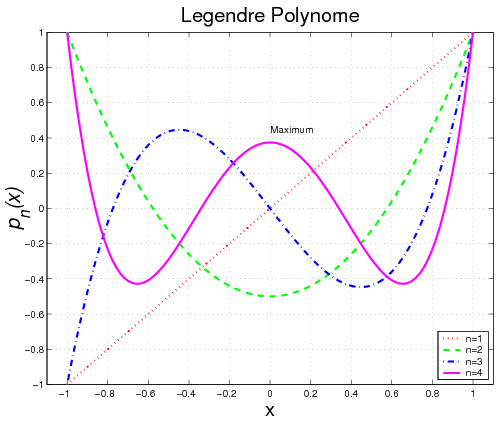
\includegraphics[width=0.5\textwidth]{figures/grafik_5}\hfil
%\end{columns}
\end{frame}
% 
% Slide
% 
%\begin{frame}[fragile]{Umgang mit Grafikfenster}
%\begin{itemize}
%\item Öffnen eines (weiteren) Grafikfensters: \alert{\imatlab{figure}}.  Eine
%  Grafik wird immer im aktuellen Fenster erzeugt. Ist noch kein
%  Fenster geöffnet, so wird ein Fenster erzeugt.
%\item Durch den Befehl \alert{\imatlab{hold on}} werden bestehende Grafiken im
%  aktuellen Fenster erhalten. Neue Grafiken werden den bestehenden
%  hinzugefügt. 
%\item \alert{\imatlab{hold off}} (default) überschreibt Grafiken im
%  aktuellen Fenster
%\item Schliessen: \alert{\imatlab{close}}, \alert{\imatlab{close all}}
%\end{itemize}
%\end{frame}


\subsection{Weitere zweidimensionale Darstellungsmöglichkeiten}

% 
% Slide
% 
\begin{frame}[fragile]{Darstellung von Daten}
\begin{itemize}
\item Balkendiagramm:
\begin{matlabin}
bar(<Daten>) 
\end{matlabin}
\item Histogramm: 
\begin{matlabin}
hist(<Daten>,<Anzahl Bars>)
\end{matlabin}
\item einfacher ausgefüllter Plot: 
\begin{matlabin}
area(<x>,[<y1>,<y2>])
\end{matlabin}
(y1 und y2 werden addiert)
\begin{pyin}
fill(<x>,<y1>)+fill_between(<x>,<y2>,<y1>)
\end{pyin}
\item Tortengrafik: 
\begin{matlabin}
pie3([<anteil1> <anteil2> .. <anteilx>])
  \end{matlabin}
\begin{pyin}
pie([<anteil1>,<anteil2> .. <anteilx>])  
\end{pyin}
\end{itemize}
\end{frame}
% 
% Slide
% 
\begin{frame}[fragile]{Matlab: Darstellung von Daten}
\begin{center}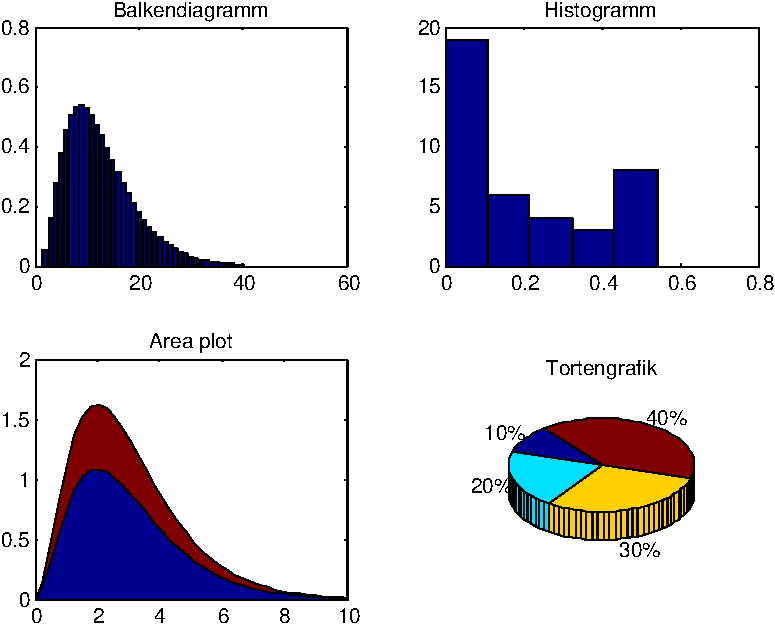
\includegraphics[height=0.8\textheight]{figures/darstellung_daten_2d}\end{center}
\end{frame}
% 
% Slide
% 
\begin{frame}[fragile]{Matlab: Darstellung von Daten}
\begin{matlabin}
n = linspace(0,10,40);
y = n.^2.*exp(-n);

% Balkendiagramm
subplot(2,2,1),
bar(y); title('Balkendiagramm');

% Histogramm
subplot(2,2,2),
hist(y,5); title('Histogramm');

% Area plot
subplot(2,2,3),
area(n,[y',2*y']); title('Area plot');

% Tortengrafik
subplot(2,2,4),
pie3([ 1 2 3 4]); title('Tortengrafik');
\end{matlabin}
\end{frame}
% 
% Slide
% 
\begin{frame}[fragile]{Python: Darstellung von Daten}
\begin{center}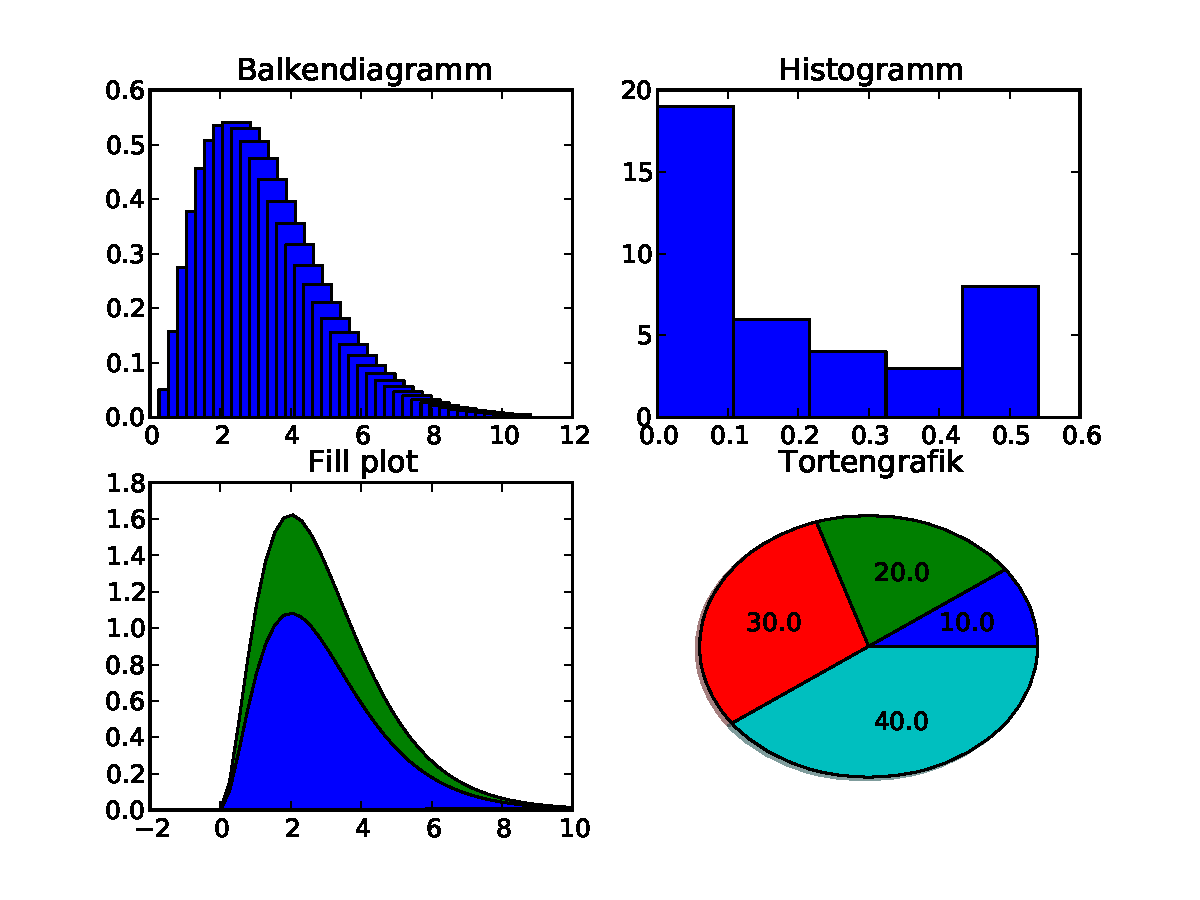
\includegraphics[height=0.8\textheight]{figures/darstellung_daten_2d_py}\end{center}
\end{frame}

% 
% Slide
% 
\begin{frame}[fragile]{Python: Darstellung von Daten}
\begin{pyin}
n = linspace(0,10,40)
y = n**2.*exp(-n)

#Balkendiagramm
subplot(2,2,1)
bar(n,y),title('Balkendiagramm')

#Histogramm
subplot(2,2,2)
hist(y,5),title('Histogramm')
#Area plot
subplot(2,2,3)
fill(n,2*y),fill_between(n,3*y,2*y,facecolor='green')
title('Fill plot')
#Tortengrafik
subplot(2,2,4)
pie([ 1,2,3,4],autopct='%1.1f', shadow=True)
title('Tortengrafik')
\end{pyin}
\end{frame}
% 
% Slide
% 
\begin{frame}[fragile]{Approximation von Integralen}
Approximiere $\int_0^1 f(x) dx$ durch (Mittelpunktsregel)
{\scriptsize \[ \int_0^1 f(x) dx \approx  \sum_{i=1}^{N} \frac{1}{N} f \left(
\frac{i-\frac{1}{2}}{N} \right ) \]}
für gegebenes $N \in \mathbb{N}$. \textbf{Beispiel}: $f(x)=x^3$
\begin{columns}[t]
\column{0.5\textwidth}
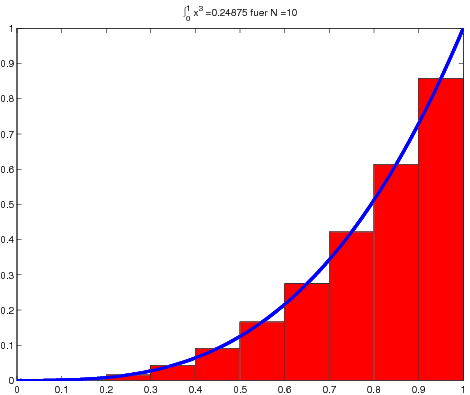
\includegraphics[width=\textwidth]{figures/integral_N=10} 
\column{0.5\textwidth}
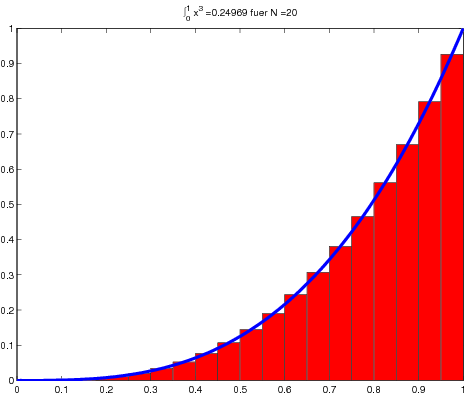
\includegraphics[width=\textwidth]{figures/integral_N=20}
\end{columns}
\end{frame}
% 
% Slide
% 
\begin{frame}[fragile]{Matlab: Integral - Implementation}
\matinput{integral.m}
\end{frame}
% 
% Slide
% 
\begin{frame}[fragile]{Python: Integral - Implementation}
  \begin{pyin}
# berechnet approximativ ein Integral 
# ueber  (0,1) durch die Mittelpunktregel
N = 10# Anzahl Unterteilungen
x = arange(0+1./(2*N),1-1./(2*N),1./N)
y = x**3
# Berechnung des Integrals
result = sum(y)*(1/N)

# Plot
for i in arange(1.,N+1):
    fill_between([(i-1)/N, i/N],[((i-0.5)/N)**3,  ((i-0.5)/N)**3],facecolor='r')
plot(arange(0,1,0.01),array(arange(0,1,0.01))**3,linewidth=3)
title('\int_0^1 x^3 = {} fuer N = {}'.format(result,N),fontsize=20)    
  \end{pyin}
\end{frame}

\subsection{Dreidimensionale Grafiken}

% 
% Slide
% 
% 
\begin{frame}[fragile]{Matlab: Dreidimensionale Grafiken}
\begin{itemize}
\item Dreidimensionale Version von \imatlab{plot}: \alert{ \imatlab{plot3}}
\item Darstellung von Funktionen $f:\mathbb{R}^2 \ \rightarrow \
  \mathbb{R}$:
\begin{itemize}
\item Contourplot (zeichnet die Niveaulinien): \alert{ \imatlab{contour}}, \alert{
    \imatlab{contourf}}, \alert{ \imatlab{contour3}}
\item Darstellung des Graphen mit Gitterlinien: \alert{ \imatlab{mesh} ,
  \imatlab{meshc}} 
\item Flächige Darstellung des Graphen: \alert{ \imatlab{surf}, \imatlab{surfc}}
\end{itemize} 
\item Darstellung von Funktionen $f:\mathbb{R}^3 \ \rightarrow \
  \mathbb{R}$:
\begin{itemize}
\item Streifenansichten \alert{ \imatlab{slice}}
\end{itemize}
\end{itemize}
\alert{ \imatlab{mesh(X,Y,Z)}} z.B. stellt für Matrizen $X,Y,Z \in
\mathbb{R}^{n \times k}$ die Punkte 
\[\alert{  (X(i,j), Y(i,j), Z(i,j))} \quad \mbox{dar.}\]
\end{frame}

\begin{frame}[fragile]{Python: Dreidimensionale Grafiken}
3D Grafiken können auf sehr verschiedene Weise erzeugt werden:
  \begin{itemize}
    \item \alert{Mayavi mlab} (gute 3D Beschleunigung, GUI möglich, Empfohlen)
  \item \alert{mplot3d} (keine 3D Beschleunigung, am einfachsten zu Benutzen) 
  \item \alert{easyviz} aus den scitools (Frontend zu diversen Tools)
\end{itemize}
Allen Tools ist es gemein, dass sie versuchen Matlab-Syntax nahe zu kommen.
Aufgrund der Vielfalt wird hier aber auf einer Auflistung der Befehle verzichtet.

Wir benutzen \alert{mplot3d}, es sei denn es etwas Anderes angegeben.\\
Import-Zeile: \isage{from mpl_toolkits.mplot3d import Axes3D}
\end{frame}
% 
% Slide
% 
\begin{frame}[fragile]{3D Kurven}
Bei gegebenen Vektoren $x=(x_i)_{i=1}^n$, $y=(y_i)_{i=1}^n$,
$z=(z_i)_{i=1}^n$ erzeugt \alert{ \imatlab{plot3(x,y,z)}} einen Plot der die Punkte
$(x_i,y_i,z_i)$ und $(x_{i+1},y_{i+1},z_{i+1})$ miteinander
verbindet. \\
\begin{center}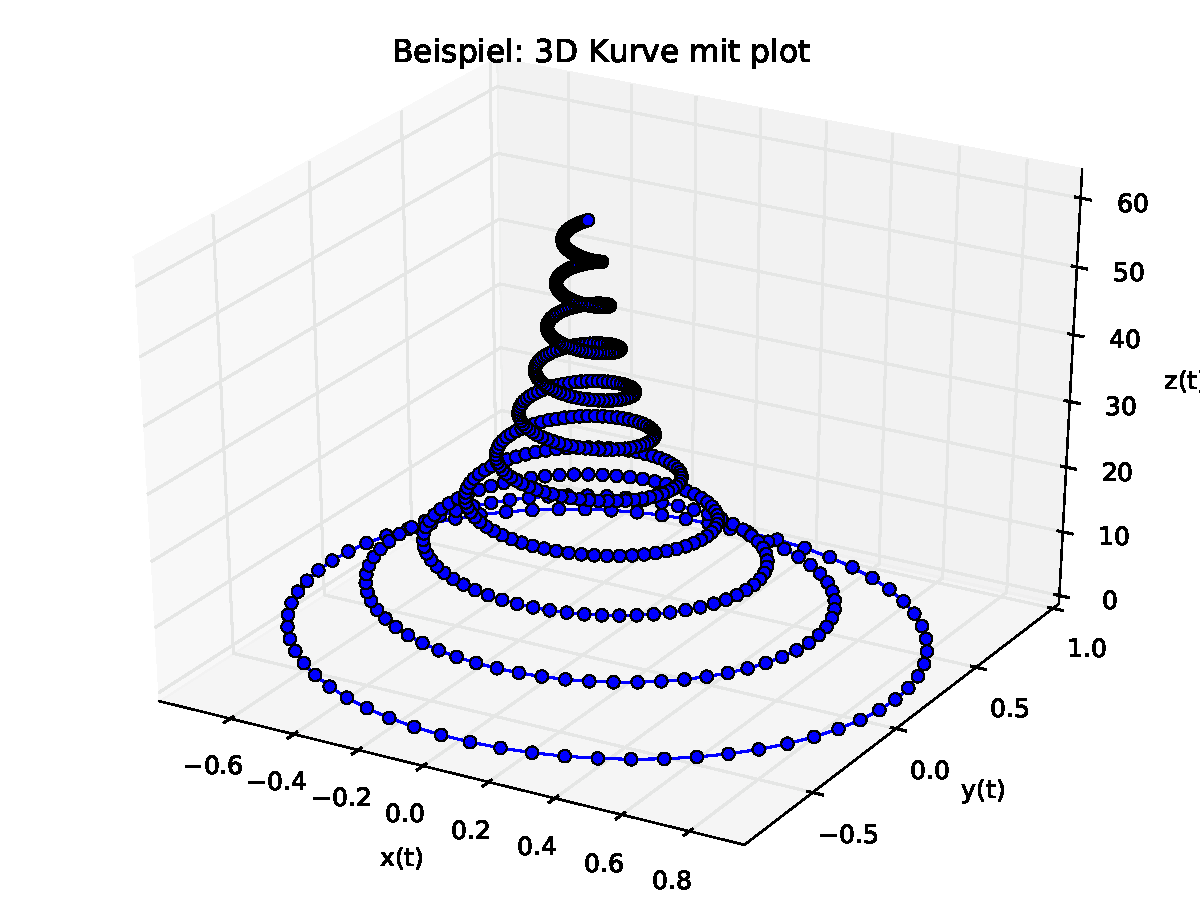
\includegraphics[width=0.6\textwidth]{figures/plot3d_py}\end{center}
\end{frame}
% 
% Slide
% 
\begin{frame}[fragile]{Beispiel 3D Kurven}
\begin{matlabin}
t = 0:0.1:20*pi;
x = exp(-t/20).*sin(t);
y = exp(-t/20).*cos(t);
z = t;
plot3(x,y,z,'b-o','LineWidth',1);
xlabel('x(t)'), ylabel('y(t)');
 zlabel('z(t)');
title('Beispiel: 3D Kurve mit plot3','FontSize',15);
\end{matlabin}
\begin{pyin}
t = arange(0,20*pi,0.1)
x = exp(-t/20)*sin(t)
y = exp(-t/20)*cos(t)
z = t
fig=figure()
ax = Axes3D(fig)
plot(x,y,z,'b-o',linewidth=1)
ax.set_xlabel('x(t)'),ax.set_ylabel('y(t)'),ax.set_zlabel('z(t)')
title('Beispiel: 3D Kurve mit plot',fontsize=15)  
\end{pyin}
\end{frame}
% 
% Slide
% 
\begin{frame}[fragile]{Blickwinkel}
  \centering \imatlab{view(az,el)}(Matlab)| \isage{Axes3D.view_init(el,az)}(Python)
\begin{itemize}
\item \alert{ \imatlab{az}} ist die horiz. Rotation in Grad (Def. \alert{
  $-37.5$}) 
\item \alert{ \imatlab{el}} ist die vertikale Rotation in Grad (Def. \alert{
  $30$})
\end{itemize}
\begin{center}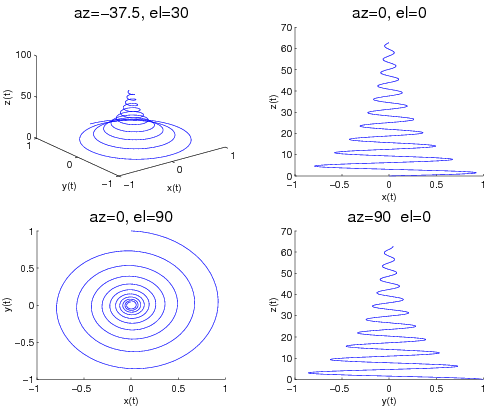
\includegraphics[width=0.6\textwidth]{figures/beispiel_plot3_2}\end{center}
\end{frame}
% 
% Slide
% 
\begin{frame}[fragile]{3D-Funktionenplots}

Darstellung von Funktionen
\[ f: \mathbb{R}^2 \quad  \rightarrow \quad \mathbb{R} \]
\hspace*{1cm}\\

\textbf{Beispiel:}\\
\alert{ \[ f(x,y):=\exp(-x^2-y^2)\sin(\pi x y) \]}
\end{frame}
% 
% Slide
% 
\begin{frame}[fragile]{Matlab: Funktionenplot}
\hfil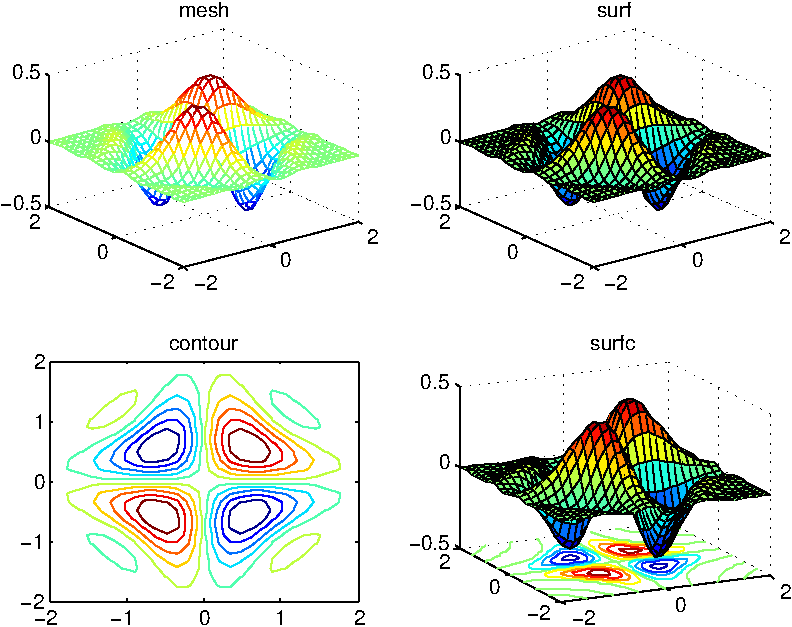
\includegraphics[width=0.8\textwidth]{figures/beispiel_function_plot_3d}\hfil
\end{frame}
% 
% Slide
% 
\begin{frame}[fragile]{Matlab: Funktionenplot - Implementation}
\begin{matlabin}
% Erzeugen des Gitters
x = linspace(-2,2,30);
y = linspace(-2,2,30);
[X,Y] = meshgrid(x,y);
% Funktionswerte
Z = exp(-X.^2-Y.^2).*sin(pi*X.*Y);

% verschiedenen Darstellungen
subplot(2,2,1),
 mesh(X,Y,Z), title('mesh');
subplot(2,2,2),
 surf(X,Y,Z), title('surf');
subplot(2,2,3),
 contour(X,Y,Z,10), title('contour');
subplot(2,2,4),
 surfc(X,Y,Z);
 view(-26,20), title('surfc');
\end{matlabin}
\end{frame}
% 
% Slide
% 
\begin{frame}[fragile]{Python: Funktionenplot}
\hfil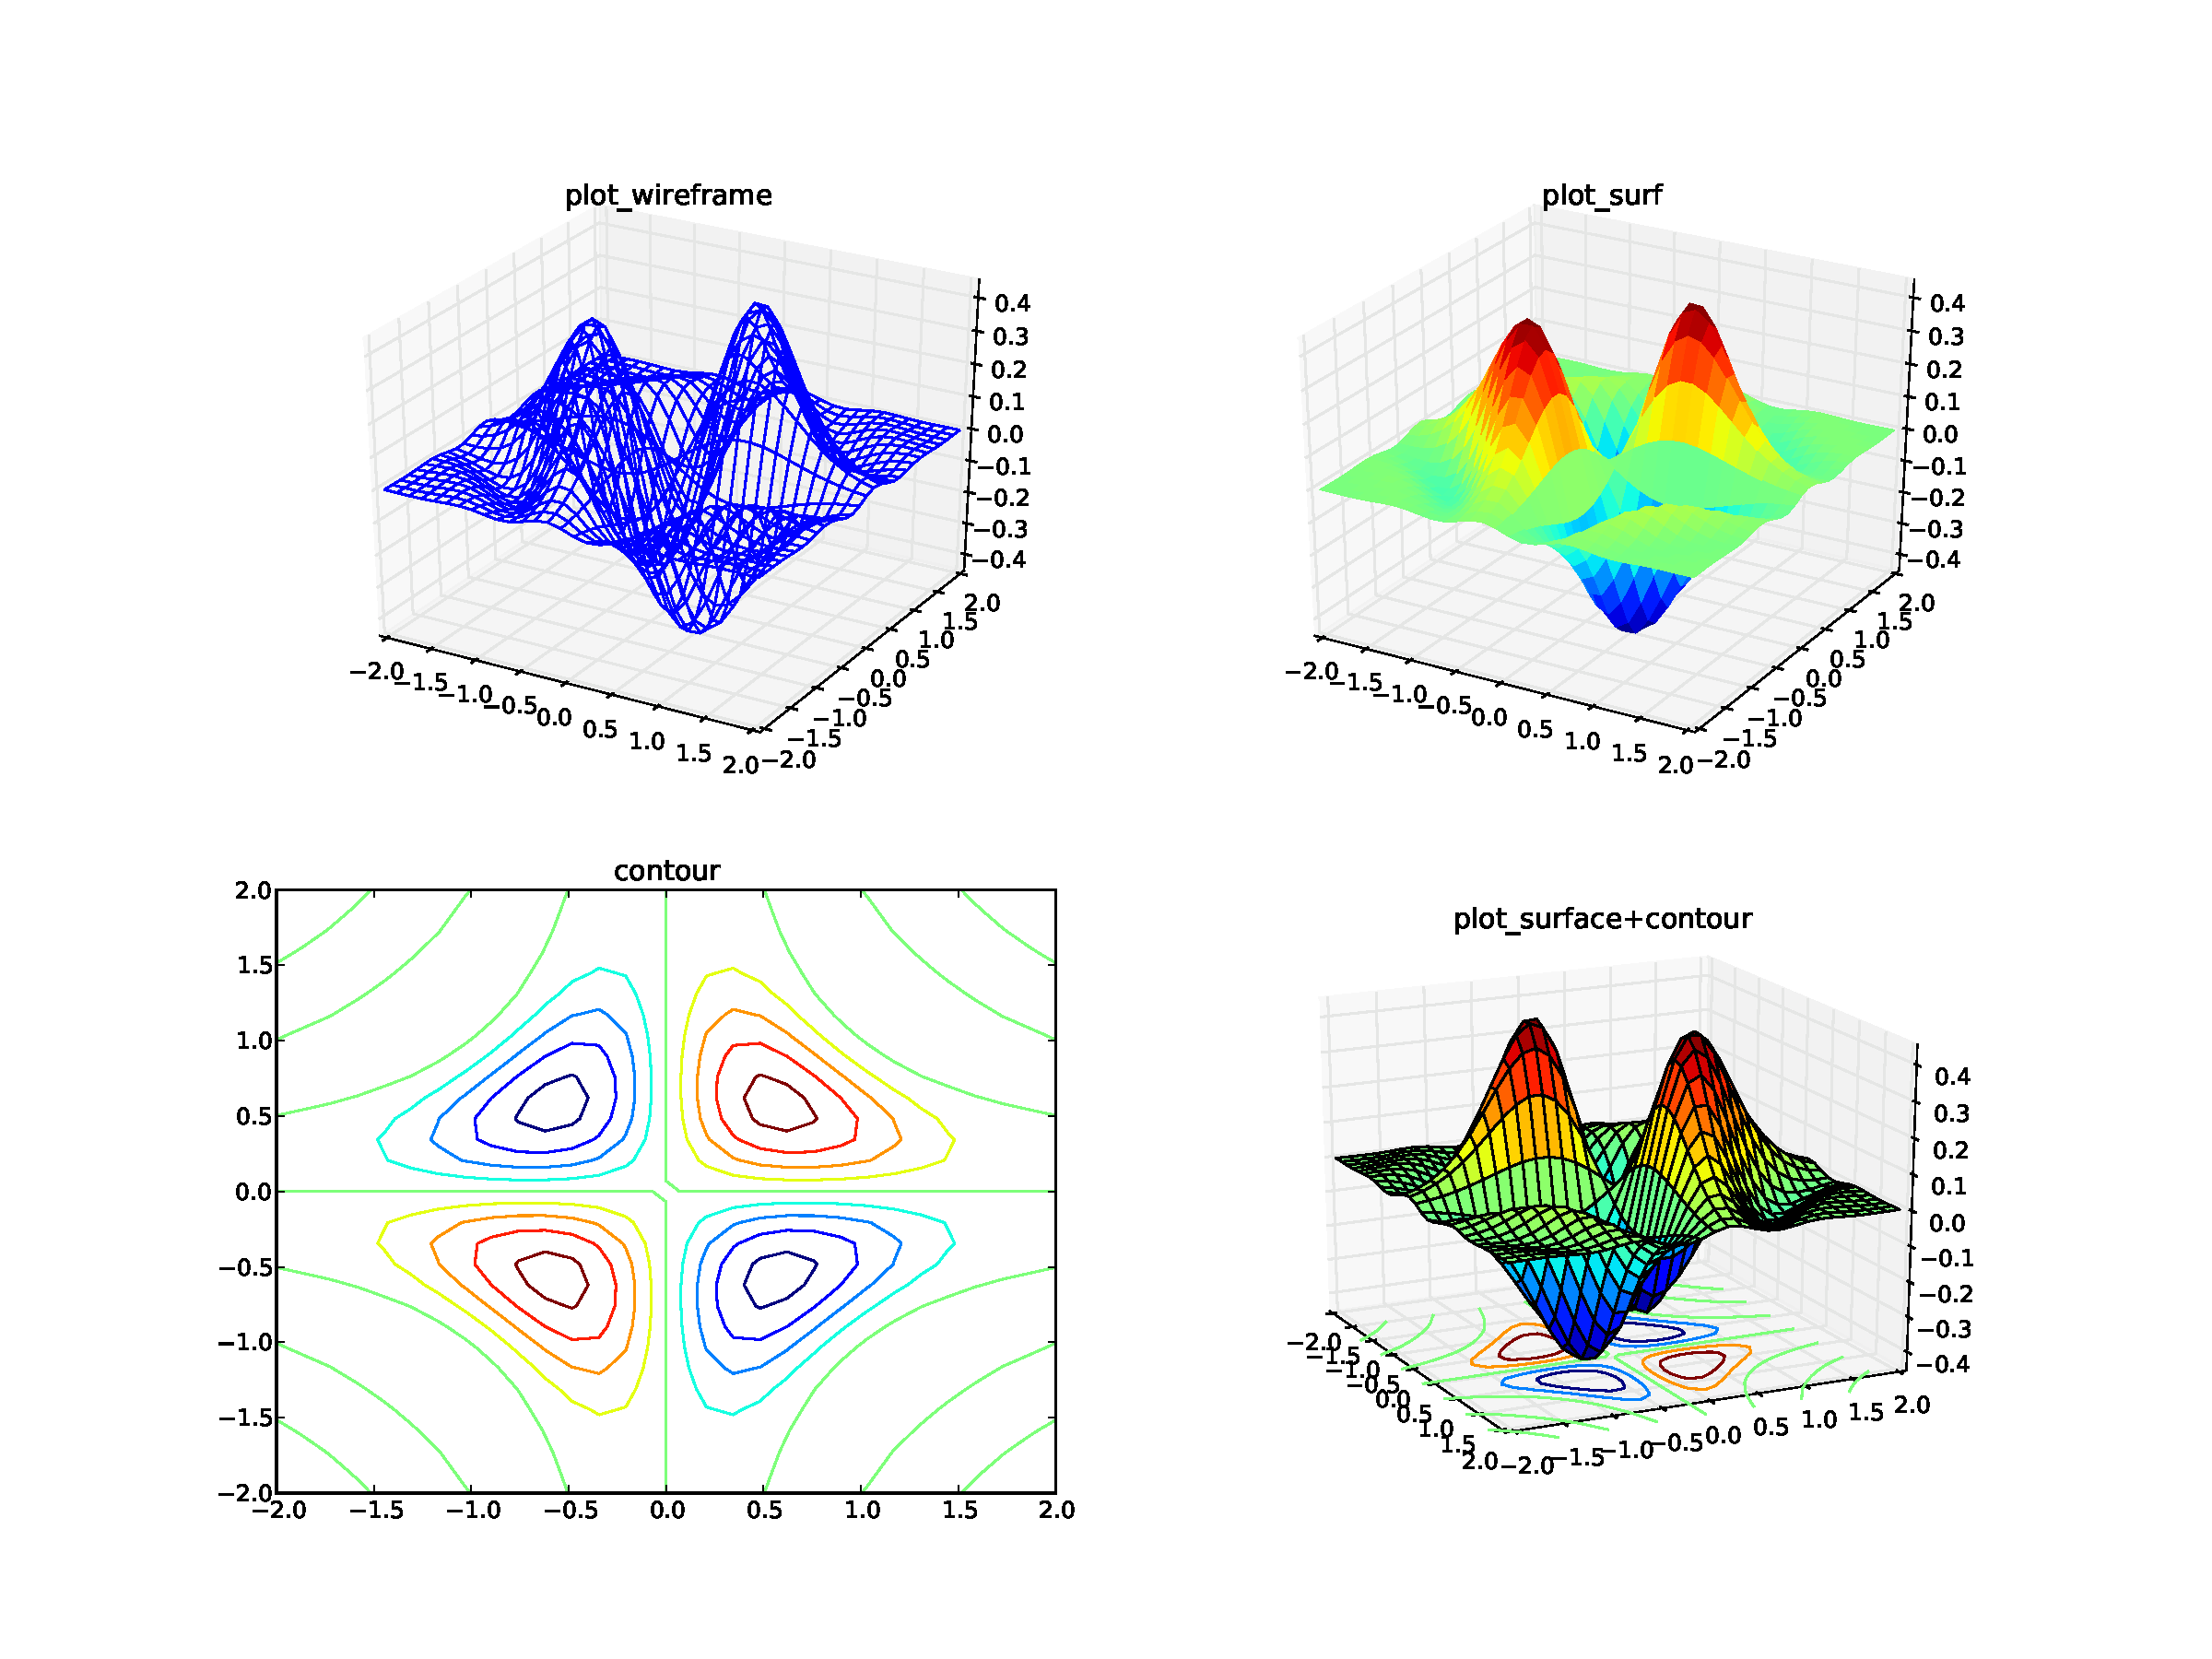
\includegraphics[width=0.8\textwidth]{figures/function_plot3d_py}\hfil
\end{frame}

% 
% Slide
% 
\begin{frame}[fragile]{Python: Funktionenplot - Implementation}
  \begin{pyin}
x = linspace(-2,2,30)
y = linspace(-2,2,30)
[X,Y] = meshgrid(x,y)
Z = exp(-X**2-Y**2)*sin(pi*X*Y)
fig=figure()
ax = fig.add_subplot(2, 2, 1, projection='3d')
ax.plot_wireframe(X,Y,Z),title('plot_wireframe')

ax = fig.add_subplot(2, 2, 2, projection='3d')
ax.plot_surface(X,Y,Z,rstride=1,cstride=1,cmap=cm.jet,linewidth=0),title('plot_surface')

subplot(2, 2, 3)
contour(X,Y,Z,10), title('contour')

ax = fig.add_subplot(2, 2, 4, projection='3d') 
ax.plot_surface(X,Y,Z,rstride=1,cstride=1,cmap=cm.jet)
ax.contour(X, Y, Z, zdir='z', offset=-0.5)
ax.view_init(20,-26),title('plot_surface + contour')    
  \end{pyin}
\end{frame}

% 
% Slide
% 
\begin{frame}[fragile]{subplot}
\begin{matlabin}
subplot(<n>,<m>,<k>)
\end{matlabin}
zerlegt das Grafikfenster in $n \times m$ Teilfenster. 

Die Zahl $1
\leq k \leq nm$ gibt an, welches Teilfenster gerade aktiv
ist. \\

Durchnumeriert wird zeilenweise, also $(1,1), (1,2), \dots$.

\alert{Python-Zusatz (mplot3d):} Für die mplot3d-Achsen braucht man folgenden subplot:
\begin{pyin}
fig.add_subplot(<n>, <m>, <k>, projection='3d')
\end{pyin}
\end{frame}

% 
% Slide
% 
\begin{frame}[fragile]{meshgrid}
Zu Vektoren $x=(x_i)_{i=1}^k$, $y=(y_j)_{j=1}^n$ erzeugt 
\begin{matlabin}
[X,Y]=meshgrid(x,y)
\end{matlabin}
Matrizen $X,Y \in \mathbb{R}^{n \times k}$, wobei jede Zeile von $X$
eine Kopie des Vektors $x$ ist und $Y$ als Spalten den Vektor $y$
enthält. \\
Dann hat \alert{ \imatlab{Z=X.*Y}} die Komponenten 
\[ Z(i,j)=x(j)*y(i). \]
\end{frame}

%\end{frame}
% 
% Slide
% 
%\begin{frame}[fragile]{Weitere Möglichkeiten}
%\begin{itemize}
%\item Darstellung versteckter Linien (bei \imatlab{mesh}): \alert{ \imatlab{hidden off}}, Default:
%\alert{ \imatlab{hidden on}}
%\item Verschmieren des Gitters: \alert{ \imatlab{shading('interp')}}
%\item Blickwinkel: \alert{ \imatlab{view(az,el)}}
%\item ähnlich wie \imatlab{mesh}; nur mit 'Vorhang': \alert{
%  \imatlab{meshz(X,Y,Z)}}
%\end{itemize}
%\end{frame}
% 
% Slide
% 
%\begin{frame}[fragile]{Beispiel: Funktionenplot}
%\hfil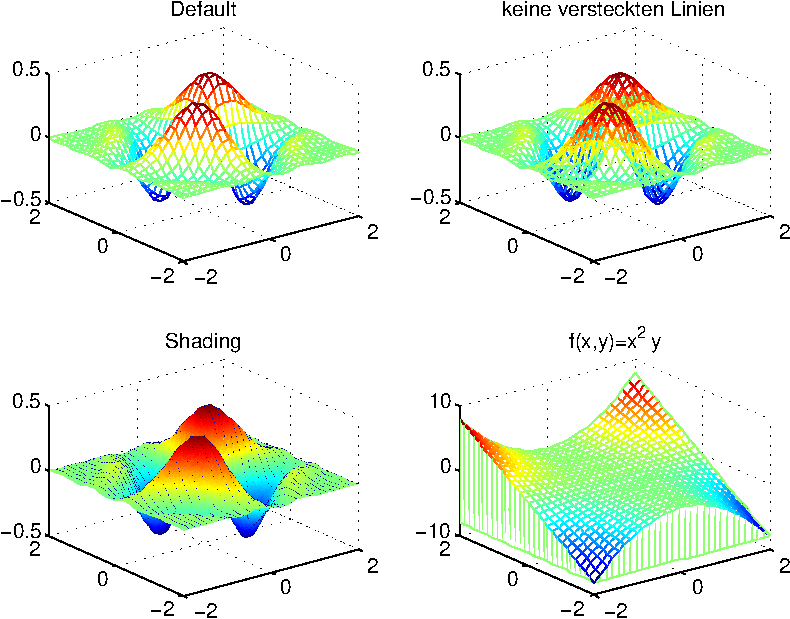
\includegraphics[width=0.8\textwidth]{figures/beispiel_function_plot_3d_2}\hfil
%\end{frame}
% 
% Slide
% 
%\begin{frame}[fragile]{Funktionenplot - Listing}
%\begin{matlabin}
%x = linspace(-2,2,30);
%y = linspace(-2,2,30);
%[X,Y] = meshgrid(x,y);
%% Funktionswerte
%Z = exp(-X.^2-Y.^2).*sin(pi*X.*Y);
%
%% verschiedenen Darstellungen
%subplot(2,2,1),
% mesh(X,Y,Z), title('Default');
%subplot(2,2,2),
% mesh(X,Y,Z), hidden off,
% title('keine versteckten Linien');
%subplot(2,2,3), surf(X,Y,Z);
% shading('interp'), title('Shading');
%subplot(2,2,4), Z=X.^2.*Y;
% meshz(X,Y,Z), title('f(x,y)=x^2 y');
%\end{matlabin}
%\end{frame}

% 
% Slide
% 
\begin{frame}[fragile]{Matlab: Contour Plots}
\hfil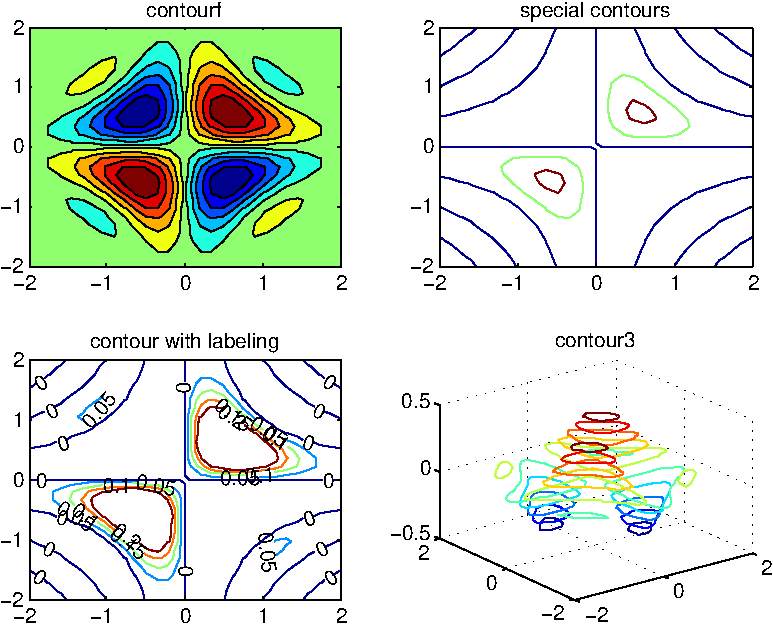
\includegraphics[width=0.8\textwidth]{figures/beispiel_function_plot_contour}\hfil
\end{frame}
% 
% Slide
% 
\begin{frame}[fragile]{Matlab: Contour Plots - Listing}
\matinput{contour_plot.m}
\end{frame}
% 
% Slide
% 
\begin{frame}[fragile]{Contour-Befehle}
\begin{itemize}
  \item \imatlab{[C,h] = contour(X,Y,Z,n)}| \isage{C = contour(X,Y,Z,n)}\\ 
    zeichnet f\"ur $n\in \mathbb{N}$
  $n$-Konturlinien. Ist $n$ ein Vektor, werden Konturlinien zu den Werten in
  dem Vektor $n$ geplottet. (C sind die Konturlinien und h ist das Grafik-handle).
\item \imatlab{contourf(X,Y,Z,n)}\\
  funktioniert wie \imatlab{contour} nur das die Flächen
  zwischen den Konturlinien ausgefüllt werden.
\item \imatlab{clabel(C,h)} (Matlab)| \isage{clabel(C, inline=1)}(Python)\\ 
  beschriftet die Konturlinien, deren Werte in $C$
  gespeichert sind und die zum Grafik-Handle $h$ gehören.
\item \imatlab{contour3(X,Y,Z,n)}| \isage{Axes3D.contour(X,Y,Z,n)}(Python)\\  
  zeichnet jede Konturlinie auf einer anderen H\"ohe.
\end{itemize}
\end{frame}
% 
% Slide
% 
\begin{frame}[fragile]{Python: Contour Plots}
\hfil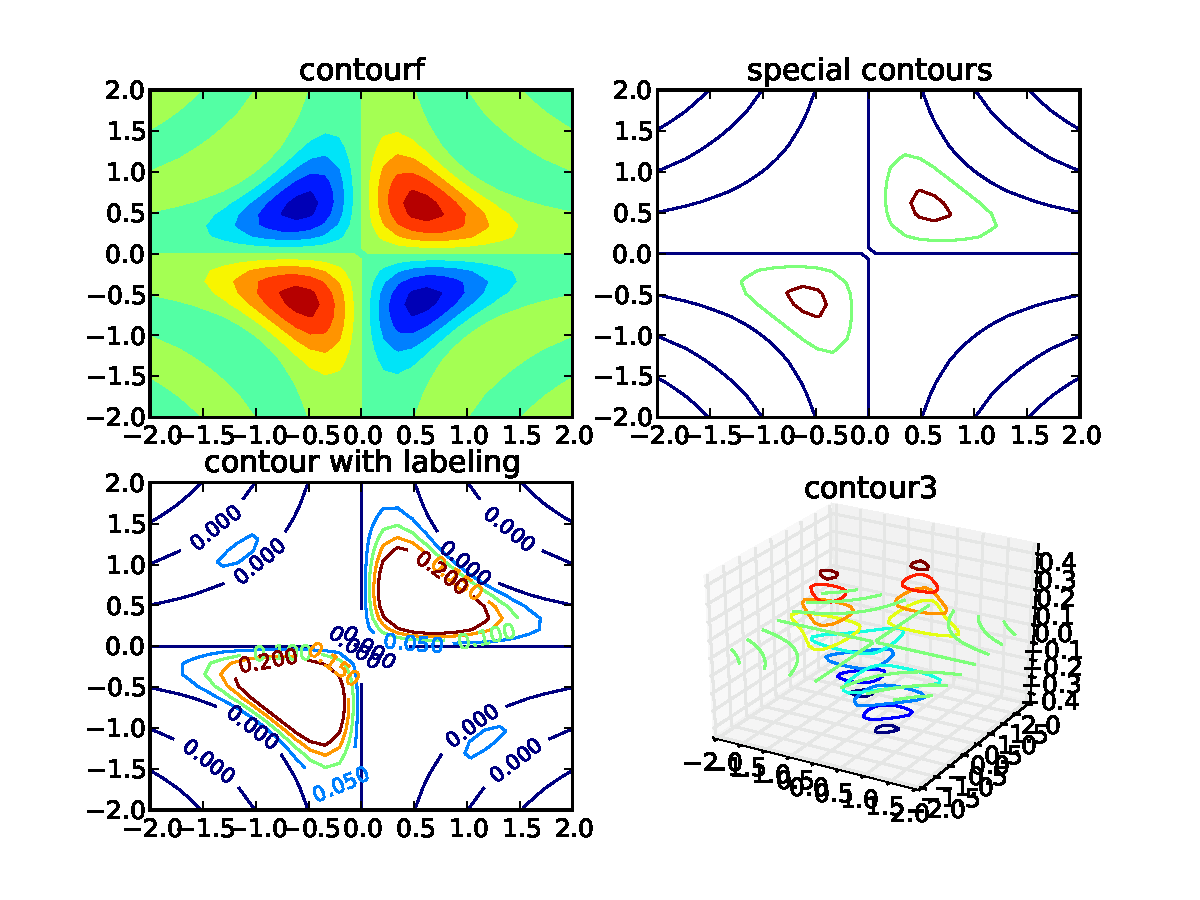
\includegraphics[width=1\textwidth]{figures/function_plot_contour_py}\hfil
\end{frame}
% 
% Slide
% 
\begin{frame}[fragile]{Python: Contour Plots - Listing}
  \begin{pyin}
# Erzeugen des Gitters
x = linspace(-2,2,30)
y = linspace(-2,2,30)
[X,Y] = meshgrid(x,y)
# Funktionswerte
Z = exp(-X**2-Y**2)*sin(pi*X*Y)
# verschiedene Darstellungen
fig=figure()
subplot(2,2,1)
contourf(X,Y,Z,10), title('contourf')
subplot(2,2,2)
contour(X,Y,Z,[0,0.2,0.4]), title('special contours')
subplot(2,2,3)
CS = contour(X,Y,Z,[0,0.05,0.1,0.15,0.2])
plt.clabel(CS, inline=1, fontsize=10)
title('contour with labeling')
ax = fig.add_subplot(2, 2, 4, projection='3d')
ax.contour(X,Y,Z,10),title('contour3')    
  \end{pyin}
\end{frame}

%
% Slide
% 
\begin{frame}[fragile]{Matlab: Slice}
\begin{matlabin}
slice(X,Y,Z,V,sx,sy,sz)
\end{matlabin}
zeichnet  Schnitte zu den Funktionswerten $V(i)$ zu
$(X(i),Y(i),Z(i))$. Schnitte sind durch die Vektoren $sx$, $sy$ und $sz$
gegeben.\\
\textbf{Beispiel}: \alert{ \[ f(x,y,z):=\exp(-x^2-y^2)\sin(\pi x y z) \]}
\matinput{beispiel_slice.m}
\end{frame}

\begin{frame}[fragile]{Matlab: Beispiel-slice}
\hfil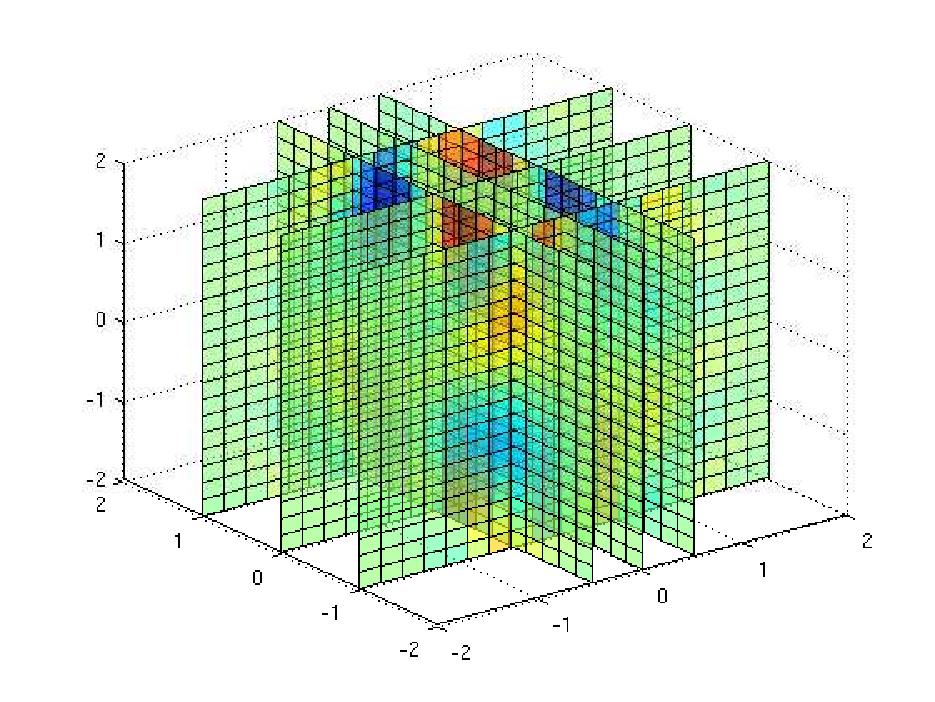
\includegraphics[width=0.8\textwidth]{figures/slice}\hfil
\end{frame}

\begin{frame}[fragile]{Python: slice (Mayavi mlab)}
  \begin{pyin}
ml.pipeline.image_plane_widget(ml.pipeline.scalar_field(V), plane_orientation=<'x_axes'|'y_axes'|'z_axes'>, slice_index=<idx>)    
  \end{pyin}
  \begin{itemize}
    \item V: Funktionswerte $V(i)$ zu $(X(i),Y(i),Z(i))$.
    \item \isage{plane_orientation}: Schnitte durch x-/y-/z-Achse
    \item \isage{slice_index}: Index in den Matrizen (keine direkte Koordinaten-Angabe)
  \end{itemize}

  \begin{pyin}
X, Y, Z = np.ogrid[-2:2:20j,-2:2:20j,-2:2:20j]
V = exp(-X**2-Y**2) * sin(pi*X*Y*Z)
ml.pipeline.image_plane_widget(ml.pipeline.scalar_field(V), plane_orientation='x_axes', slice_index=8)
ml.pipeline.image_plane_widget(ml.pipeline.scalar_field(V), plane_orientation='y_axes', slice_index=5)
ml.pipeline.image_plane_widget(ml.pipeline.scalar_field(V), plane_orientation='y_axes', slice_index=15)    
  \end{pyin}

\end{frame}

\begin{frame}[fragile]{Python: Beispiel-slice}
\hfil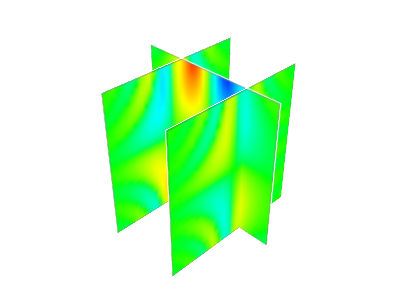
\includegraphics[width=0.8\textwidth]{figures/pyslice}\hfil
\end{frame}

\subsection{Animation}
% 
% Slide
% 
\begin{frame}[fragile]{Matlab: Animation-Beispiel}
\matinput{animation.m}
\end{frame}
%
% Slide
% 
\begin{frame}[fragile]{Matlab: Erstellen einer Animation/Videos}
\begin{itemize}
\item \alert{\imatlab{F(j)=getframe}}\\
aktuelle Grafik in das Array $F$ speichern.
\item \alert{\imatlab{movie(F,n,fps)}}\\
Sequenz der Bilder $F$ darstellen. wobei $n$ die Anzahl der Wiederholungen angibt und $fps$ der
  gezeigten Frames pro Sekunde entspricht (Default: $n=1$, $fps=12$). 

\item \alert{\imatlab{movie2avi(F,Dateiname)}}\\
Speichern des Movies in AVI Format: \end{itemize}
\end{frame}
% 
% Slide
% 
\begin{frame}[fragile]{Python: Animation-Beispiel}
  \begin{pyin}
[X,Y] = meshgrid(arange(-1,1,0.05),arange(-1,1,0.05))
fig = figure()
ax = Axes3D(fig)

for j in arange(1,50):
    Z = cos(j**0.5*pi*exp(-X**2-Y**2))
    ax.plot_surface(X,Y,Z,rstride=1,cstride=1,cmap=cm.jet,linewidth=0)
    ax.grid(b=False)
    fname = '/scratch/jschulz1/_tmp{:05d}.png'.format(j) 
    fig.savefig(fname)
    ax.cla()
    
print ("creating movie")
CreateMovie('/scratch/jschulz1/','course', 10)    
  \end{pyin}
\end{frame}

%
% Slide
%


\end{document}




